\documentclass[12pt]{article}

\usepackage[english]{babel}
\usepackage[utf8]{inputenc}
\usepackage{fancyhdr}

\usepackage[margin=1in]{geometry}
\usepackage{siunitx}
\usepackage{tikz}
\usepackage{float}
\usepackage{amsmath}
\usepackage{enumitem}

\usepackage[font=small,labelfont=bf]{caption}
\usepackage[nodisplayskipstretch]{setspace}

\usetikzlibrary{scopes}
\usetikzlibrary{angles,quotes}
\usetikzlibrary{calc}
\graphicspath{ {/} }

\newcommand*{\I}{\imath}
\newcommand*{\J}{\jmath}
\newcommand{\norm}[1]{\lvert #1 \rvert}

\setlist[enumerate, 1]{label=\alph*.}

\begin{document}
\sisetup{per-mode=symbol}

\begin{titlepage}
    \begin{center}
        \vspace*{1cm}
        \textbf{PV Diagrams and Work}

        \vspace{0.5cm}
        Lab: 02

        \vspace{1cm}

        \textbf{Jaden Moore}

        \vfill

        Orange Coast College\\
        Physics A285L\\
        September 27th, 2021

    \end{center}
\end{titlepage}

\pagestyle{fancy}
\fancyhf{}
\setlength{\headheight}{15pt}
\lhead{PV Diagrams and Work}
\rhead{Lab: 02}
\cfoot{\thepage}

\section{Introduction}
In this lab, we analyze the behavior of various gases using a pressure-volume diagram. First we analyze the change in internal energy $\Delta U$ for each gas as the temperature changes. We then gather and compare the experimental values of work done by the gas with the theoretical values to retrieve a percent error between the two.

\section{PV Diagrams and Work}
Consider the experiment provided by Physlet\textregistered \space Physics Exploration 20.5: PV Diagrams and Work. Below we show the pressure-diagram of an adiabatic gas,

\begin{figure}[H]
    \begin{center}
        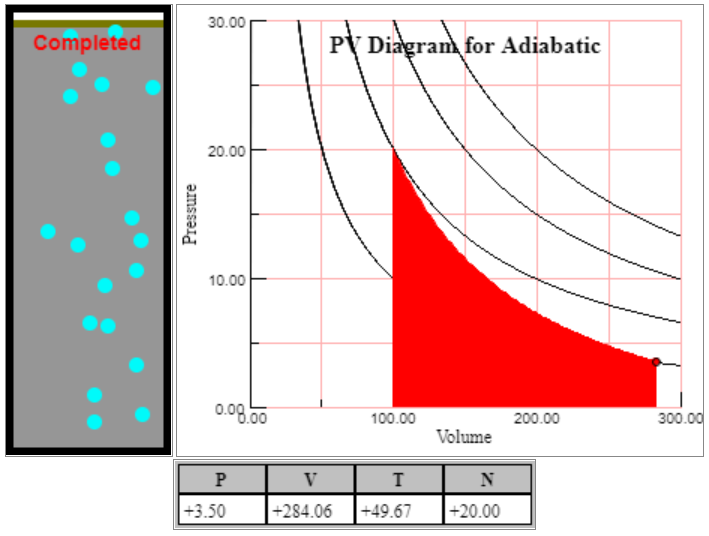
\includegraphics[scale=0.5]{Figure-1.png}
        \caption {pressure-volume diagram of adiabatic gas}
    \end{center}
\end{figure}

From the graph, we see that the area under the graph is equal to the work done by the gas, that is

\begin{equation}
    \begin{split}
        W &= \int{P}dV
    \end{split}
\end{equation}
Below we put into a table the various initial and final states of the three gases which were recorded from the pressure-volume diagram in the experiment.

\newcolumntype{P}[1]{>{\centering\arraybackslash}p{#1}}

\setlength{\tabcolsep}{3pt}
\renewcommand{\arraystretch}{1.25}

\begin{figure}[H]
    \begin{center}
        \begin{tabular}{ P{2cm}| P{2cm} P{2cm} P{2cm} P{2cm} P{2cm} P{2cm} P{2cm} }
            \hline
            \multicolumn{8}{c}{Table 1: Initial and final values of the gases [Experiment contains no units]} \\

            \hline
            gas       & $P_i$ & $P_f$ & $V_i$ & $V_f$  & $T_i$ & $T_f$ & $N$                                  \\
            \hline
            isobaric  & 20    & 20    & 100   & 48.33  & 100   & 48.33 & 20                                   \\
            isochoric & 20    & 9.80  & 100   & 100    & 100   & 49    & 20                                   \\
            adiabatic & 20    & 3.50  & 100   & 284.06 & 100   & 49.67 & 20                                   \\
            \hline
        \end{tabular}
    \end{center}
\end{figure}

(1) Through the analysis of the pressure-volume diagrams for isobaric, isochoric, and adiabatic gases, we can calculate the change in internal energy $\Delta U$ where $\Delta U = \frac{3}{2}N\Delta T$ where $N$ is the number of moles and $\Delta T$ is the change in temperature. From the experiment, we get that

\begin{equation*}
    \begin{split}
        \Delta U_{isobaric} &= \frac{3}{2}N(T_f - T_i) = \frac{3}{2}(20)(\SI{48.33}{\degreeCelsius} - \SI{100}{\degreeCelsius}) = \SI{-1550.1}{J} \\
        \Delta U_{isochoric} &= \frac{3}{2}N(T_f - T_i) = \frac{3}{2}(20)(\SI{49}{\degreeCelsius} - \SI{100}{\degreeCelsius}) = \SI{-1530}{J} \\
        \Delta U_{adiabatic} &= \frac{3}{2}N(T_f - T_i) = \frac{3}{2}(20)(\SI{49.67}{\degreeCelsius} - \SI{100}{\degreeCelsius}) = \SI{-1509.9}{J}
    \end{split}
\end{equation*}

\bigskip

(2) From the diagram, we can estimate the work done by each gas by estimating the area under the curve. We note that from the experiment, one box on the graph is equal to $50 \text{ (volume)}$ x $5 \text{ (pressure)}$ = 250 area. That is,

\begin{equation*}
    \begin{split}
        W_{isobaric} &\approx -4 (box) = -4(250) = \SI{-1000}{J} \\
        W_{isochoric} &\approx 0 (box) = 0(250) = \SI{0}{J} \\
        W_{adiabatic} &\approx 6 (box) = 6(250) = \SI{1500}{J}
    \end{split}
\end{equation*}

We note that for the isobaric gas, the pressure stays constant, and the volume decreases, therefore it does negative work. We also notice from the diagram for the isochoric gas that the volume stays constant, so the gas does no work.

\bigskip

(3) We can then calculate the heat energy in each system and determine which gas contains the most heat. From the first law of thermodynamics we get that $Q=W + \Delta U$, that is

\begin{equation*}
    \begin{split}
        Q_{isobaric} &= W + \Delta U =  \SI{-1000}{J} + (\SI{-1550.1}{J}) = \SI{=-2550.1}{J} \\
        Q_{isochoric} &= W + \Delta U =  \SI{0}{J} + (\SI{-1530}{J}) = \SI{-1530}{J} \\
        Q_{adiabatic} &= W + \Delta U = \SI{0}{J} \\
    \end{split}
\end{equation*}

We note that for an adiabatic gas, the heat energy $Q$ is always zero. Therefore, the process which requires the most heat energy is the isobaric process. That is, for the isobaric process, we have to remove the most energy since the heat energy $Q$ is negative.

\bigskip

(4) We can calculate the theoretical values for the work done by an isobaric and adiabatic by calculating the exact area under the curve found in Equation (1). We note that for an isochoric gas, the volume is constant and thus does no work. However, for the isobaric and adiabatic gases, we get that

\begin{equation*}
    \begin{split}
        W_{isobaric} &= P(V_f - V_i) = 20(48.33 - 100) = \SI{-1033.4}{J} \\
        W_{adiabatic} &= \frac{1}{\gamma - 1}\left(P_i V_i - P_f V_f\right) = \frac{1}{\frac{5}{3} - 1}\left(20 (100) - 3.50(285.06) \right) = \SI{1508.7}{J} \\
    \end{split}
\end{equation*}

From this, we are able to calculate the percent error between the experimental work done and the theoretical work done by the gases. From this, we get that

\begin{equation*}
    \begin{split}
        \text{\% error}_{isobaric} &= \left( \frac{W_{exp} - W_{theory}}{W_{theory}} \right) 100 = \SI{-3.23}{\percent} \\
        \text{\% error}_{adiabatic} &= \left( \frac{W_{exp} - W_{theory}}{W_{theory}} \right) 100 = \SI{-0.577}{\percent} \\
    \end{split}
\end{equation*}

From this, we see that the percent error between the experimental and theoretical values for the isobaric process was within 4\% and within 1\% for the adiabatic process.

\section{Conclusion}
From this lab, we get that the area under the curve of a pressure-volume diagram is equal to the work done by the gas. Furthermore, we get that for isochoric gases, the volume stays constant, thus the work done is zero. Additionally, for adiabatic gases, the heat energy is always zero. Pressure-volume diagrams can help us better understand a type of gas and its state for various pressures and volumes.

During this lab, we did not encounter any difficulties, however we gained a greater understanding of how to read and analyze pressure-volume diagrams and how useful they can be in the study of various gases.

\end{document}